\documentclass[11pt]{article}

\usepackage[a4paper,margin=0.85in]{geometry}
\usepackage{amsmath}
\usepackage{booktabs}
\usepackage{caption}
\usepackage{graphicx}
\usepackage{tabularx}
\usepackage{url}

\emergencystretch=3em
\setlength{\parindent}{0pt}
\setlength{\parskip}{0.55em}
\captionsetup{font=small,labelfont=bf}
\renewcommand{\thesection}{S\arabic{section}}
\renewcommand{\thetable}{S\arabic{table}}
\renewcommand{\thefigure}{S\arabic{figure}}

\begin{document}

\begin{center}
{\Large\bfseries Supplementary Material}\\[0.45em]
{\large Hidden Behind the Mean: Probabilistic Thermal-Sensation Diagnostics of Discomfort-Tail Risk Under Future Weather}\\[0.45em]
Hongshan Guo et al.
\end{center}

\vspace{0.5em}
\hrule
\vspace{0.8em}

\section{Scope}

This supplementary material documents validation and reproducibility checks for the diagnostic analyses in the main manuscript. It does not report closed-loop control, energy savings, demand-response performance, or equipment-facing outcomes.

\section{Run Inventory and Trace Integrity}

The final diagnostic run contains 144 annual DOE Medium Office cases: six cities, two emissions scenarios, four time slices, and three annual weather-file severities. Each annual trace contains 35{,}040 15-minute rows and 16{,}704 occupied rows. The zone-raw trace schema contains 45 raw environmental fields: air temperature, mean radiant temperature, and relative humidity for each of 15 conditioned zones.

The final zone-raw diagnostic run produced 144 per-case trace files, 144 EnergyPlus error files, and 144 EnergyPlus end files. All annual cases completed without fatal EnergyPlus errors. Sixteen cases reported warmup load-convergence Severe messages; these cases completed successfully and are retained with this quality-assurance note.

\section{Weather Panel and Case Provenance}

The weather panel is used as a deterministic stress-test panel, not as a probabilistic climate ensemble. The 144 cases are the Cartesian product of six cities (Ahmedabad, Beijing, Guangzhou, Houston, Kolkata, and Phoenix), two emissions scenarios (SSP2-4.5 and SSP5-8.5), four time slices (baseline 2020s, near 2030s, mid 2050s, and late 2080s), and three selected annual severities (typical, hot, and heatwave-extreme). The three annual severities are selection labels within the local weather-file generation workflow; they should not be read as equal-probability climate outcomes.

The public reproducibility repository archives the run manifest, weather-file provenance table, case identifiers, trace-schema checks, and checksum records needed to audit the mapping between manuscript cases and generated annual weather files. Large weather files and per-timestep traces may be represented by checksums rather than redistributed directly where file size or third-party restrictions apply.

\section{Metabolic Profiles}

The metabolic-spread diagnostic reuses the same simulated environmental traces and re-evaluates the TSV probability model under six metabolic-load profiles: 90.0, 93.2, 100.0, 108.0, 110.0, and 120.0 W/person. Under the convention used in the manuscript, 120 W/person corresponds to 1.2 met, so the six profiles correspond to 0.900, 0.932, 1.000, 1.080, 1.100, and 1.200 met. These profiles are sensitivity cases for the reported-TSV model. EnergyPlus was not rerun with altered internal heat gains, and the profiles are not demographic strata assigned to simulated occupants.

\section{Held-Out TSV Prediction Validation}

The primary TSV predictor and the no-PMV robustness predictor were evaluated on the same held-out test partition of 22{,}223 ASHRAE Global Thermal Comfort Database II records. The split was stratified over the seven rounded TSV classes. The rounded-PMV baseline rounds PMV to the nearest TSV class and clips the value to $[-3,+3]$; it is a deterministic scalar-label baseline, not a calibrated probability model.

\begin{table}[htbp]
\centering
\caption{Held-out TSV validation for the primary predictor, no-PMV robustness predictor, and rounded-PMV class baseline.}
\label{tab:supp_tsv_validation}
\scriptsize
\setlength{\tabcolsep}{3.2pt}
\begin{tabular}{lrrrrrrr}
\toprule
Predictor & Exact (\%) & Within $\pm1$ (\%) & MAE & Tail recall (\%) & Tail F1 (\%) & Log loss & Tail MAE \\
\midrule
Primary TSV model & 47.3 & 84.1 & 0.73 & 23.4 & 34.0 & 1.454 & 0.277 \\
No-PMV TSV model & 46.9 & 83.8 & 0.73 & 23.1 & 33.5 & 1.476 & 0.278 \\
Rounded PMV class & 33.2 & 76.5 & 0.97 & 22.8 & 26.6 & -- & 0.258 \\
\bottomrule
\end{tabular}
\end{table}

\begin{table}[htbp]
\centering
\caption{Observed class support and class-specific recall on the held-out test partition. Values are percentages except support counts.}
\label{tab:supp_class_recall}
\scriptsize
\setlength{\tabcolsep}{4.2pt}
\begin{tabular}{lrrrrrrr}
\toprule
Predictor & TSV -3 & TSV -2 & TSV -1 & TSV 0 & TSV +1 & TSV +2 & TSV +3 \\
\midrule
Support ($n$) & 443 & 1238 & 3755 & 9834 & 4064 & 1982 & 907 \\
Primary TSV model & 25.5 & 6.9 & 12.4 & 88.0 & 16.2 & 15.7 & 23.9 \\
No-PMV TSV model & 23.7 & 6.5 & 13.0 & 87.4 & 15.4 & 15.8 & 23.2 \\
Rounded PMV class & 13.8 & 10.4 & 27.6 & 47.8 & 26.3 & 14.5 & 10.5 \\
\bottomrule
\end{tabular}
\end{table}

\section{Calibrated Tail-Probability Comparison}

As a scalar-reference check, PMV was also given a calibrated probability baseline. This baseline used only $|\mathrm{PMV}|$ as the input and the binary tail label $\mathbf{1}\{\mathrm{TSV}\le-2\ \mathrm{or}\ \mathrm{TSV}\ge+2\}$ as the target. An isotonic regression was fitted on the non-test partition and evaluated on the same held-out test records used in Tables~\ref{tab:supp_tsv_validation} and~\ref{tab:supp_class_recall}. This is not an ordinal TSV model; it only tests how much severe-tail probability can be recovered from PMV alone after calibration. Table~\ref{tab:supp_tail_probability_comparison} compares that scalar baseline with the primary and no-PMV TSV probability models using the same tail-probability metrics.

\begin{table}[htbp]
\centering
\caption{Held-out tail-probability comparison for the TSV probability models and the PMV-only calibrated scalar baseline. F1 is computed by screening each predicted tail probability at $p_{\mathrm{tail}}\ge0.20$.}
\label{tab:supp_tail_probability_comparison}
\scriptsize
\setlength{\tabcolsep}{3.2pt}
\begin{tabular}{lrrrrrrrrr}
\toprule
Predictor & $n$ & Mean predicted & Observed & Brier & ECE & MCE & F1 (\%) & AUROC & Avg. precision \\
\midrule
Primary TSV model & 22223 & 0.207 & 0.206 & 0.137 & 0.011 & 0.047 & 47.1 & 0.747 & 0.487 \\
No-PMV TSV model & 22223 & 0.207 & 0.206 & 0.138 & 0.006 & 0.012 & 46.4 & 0.747 & 0.483 \\
PMV-only calibrated tail baseline & 22223 & 0.206 & 0.206 & 0.161 & 0.003 & 0.017 & 32.6 & 0.571 & 0.260 \\
\bottomrule
\end{tabular}
\end{table}

The PMV-only baseline matched the overall tail prevalence after calibration, with mean predicted $p_{\mathrm{tail}}=0.206$ and observed tail frequency $0.206$. Its calibration error was low, but its discrimination was limited: AUROC was 0.571 and average precision was 0.260, compared with AUROC 0.747 and average precision 0.483--0.487 for the TSV probability models. This supports the limited interpretation in the main text: PMV contains useful scalar information, but PMV alone is not the same diagnostic object as a calibrated TSV probability distribution.

\section{Contributor-Grouped Robustness Check}

The record-level split above tests held-out records under the same overall ASHRAE-derived data distribution. As a stricter robustness check, the ordinal predictors were also re-estimated under five contributor-grouped train/calibration/test splits. Contributor groups were kept disjoint across training, calibration, and test partitions. Each split used 43 contributor groups for training, 10 for calibration, and 10 for testing; the mean test size was 26{,}484 records.

This grouped check is not used as the main model-selection criterion because contributor groups differ substantially in geography, building type, measurement protocol, and class balance. It is included to expose domain-transfer sensitivity. As expected, performance was lower than under the record-level split, especially for tail-class discrimination, but the comparison between the primary and no-PMV feature sets remained qualitatively similar.

\begin{table}[htbp]
\centering
\caption{Contributor-grouped validation over five disjoint-group splits. Values are mean (standard deviation) across splits.}
\label{tab:supp_grouped_validation}
\scriptsize
\setlength{\tabcolsep}{3.5pt}
\begin{tabular}{lrrrrrr}
\toprule
Feature set & Exact (\%) & Within $\pm1$ (\%) & Class MAE & Tail F1 (\%) & Log loss & Tail ECE \\
\midrule
Primary & 42.3 (3.0) & 80.1 (2.2) & 0.825 (0.047) & 6.1 (5.1) & 1.745 (0.222) & 0.060 (0.026) \\
No-PMV & 42.0 (3.2) & 79.4 (1.7) & 0.838 (0.042) & 4.8 (3.3) & 1.804 (0.275) & 0.057 (0.026) \\
\bottomrule
\end{tabular}
\end{table}

\section{Discomfort-Tail Probability Calibration}

The central probability variable in the manuscript is
\begin{equation}
p_{\mathrm{tail}}=\Pr(\mathrm{TSV}\le-2)+\Pr(\mathrm{TSV}\ge+2).
\end{equation}
To check whether this value behaves as a calibrated probability on held-out data, predicted $p_{\mathrm{tail}}$ values were grouped into fixed probability bins. Within each bin, the mean predicted $p_{\mathrm{tail}}$ was compared with the observed frequency of tail-class records. Tail expected calibration error (ECE) is the bin-count-weighted mean absolute difference between predicted and observed frequency. Tail maximum calibration error (MCE) is the largest bin-level absolute difference.

\begin{table}[htbp]
\centering
\caption{Held-out calibration summary for predicted discomfort-tail probability.}
\label{tab:supp_tail_calibration_summary}
\footnotesize
\setlength{\tabcolsep}{4.5pt}
\begin{tabular}{lrrrrrr}
\toprule
Predictor & $n$ & Mean predicted & Observed & Tail Brier & Tail ECE & Tail MCE \\
\midrule
Primary TSV model & 22223 & 0.207 & 0.206 & 0.137 & 0.011 & 0.047 \\
No-PMV TSV model & 22223 & 0.207 & 0.206 & 0.138 & 0.006 & 0.012 \\
\bottomrule
\end{tabular}
\end{table}

\begin{figure}[htbp]
\centering
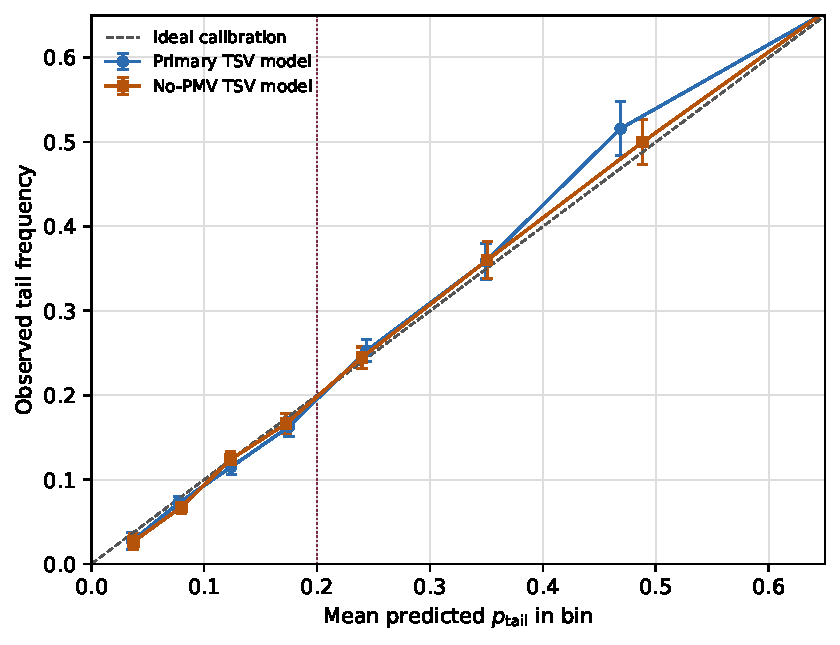
\includegraphics[width=0.68\textwidth]{figs/p_tail_calibration_reliability.pdf}
\caption{Held-out reliability check for predicted discomfort-tail probability. Points show fixed bins of predicted $p_{\mathrm{tail}}$; vertical bars show approximate 95\% binomial intervals for the observed tail frequency in each bin. The dashed line marks ideal calibration, and the dotted vertical line marks the manuscript's reporting screen $p_{\mathrm{tail}}=0.20$.}
\label{fig:supp_tail_calibration}
\end{figure}

\begin{table}[htbp]
\centering
\caption{Primary TSV model: fixed-bin held-out calibration for $p_{\mathrm{tail}}$.}
\label{tab:supp_primary_tail_bins}
\footnotesize
\begin{tabular}{lrrrr}
\toprule
Bin & $n$ & Mean predicted & Observed & Abs. error \\
\midrule
0.00--0.05 & 1024 & 0.036 & 0.027 & 0.009 \\
0.05--0.10 & 4021 & 0.077 & 0.072 & 0.005 \\
0.10--0.15 & 4652 & 0.124 & 0.115 & 0.009 \\
0.15--0.20 & 4251 & 0.175 & 0.163 & 0.012 \\
0.20--0.30 & 4277 & 0.244 & 0.253 & 0.009 \\
0.30--0.40 & 2005 & 0.350 & 0.359 & 0.009 \\
0.40--0.60 & 919 & 0.469 & 0.516 & 0.047 \\
0.60--1.00 & 1074 & 0.713 & 0.701 & 0.012 \\
\bottomrule
\end{tabular}
\end{table}

The held-out calibration check supports using $p_{\mathrm{tail}}$ as a diagnostic probability rather than only as an uncalibrated score. The primary model's mean predicted $p_{\mathrm{tail}}$ was 0.207, close to the observed held-out tail frequency of 0.206. Fixed-bin ECE was 0.011 for the primary predictor and 0.006 for the no-PMV predictor. These values do not remove the sparse-tail limitation noted in the manuscript, but they show that the aggregate tail probability is well aligned with observed tail frequency on the held-out record-level split.

\section{Generated Diagnostic Outputs}

The reproducibility workspace contains the generated outputs used by the manuscript and this supplement:
\begin{itemize}
    \item held-out TSV validation summaries and class-recall tables;
    \item contributor-grouped validation summaries for primary and no-PMV feature sets;
    \item $p_{\mathrm{tail}}$ calibration summaries, fixed-bin reliability tables, and reliability plots;
    \item scalar PMV and expected-TSV comparison diagnostics;
    \item threshold-sensitivity summaries for $p_{\mathrm{tail}}$ screens from 0.05 to 0.40;
    \item zone-aggregation summaries, zone-size mosaic inputs, and floor-position diagnostics;
    \item metabolic-spread summaries and zone-resolved metabolic-profile diagnostics;
    \item EnergyPlus trace-schema and run-quality audits.
\end{itemize}

Large per-timestep traces and third-party ASHRAE Global Thermal Comfort Database II records are not redistributed directly. The submission repository should provide scripts, processed summaries, model artifacts, weather-file provenance, and checksums for auditing the reported tables and figures where redistribution is permitted.

\end{document}
